\documentclass[10pt,a4paper,oneside,onecolumn]{article}
% PACKAGES
\usepackage[utf8]{inputenc}
\usepackage[english]{babel}
\usepackage[T1]{fontenc}
\usepackage{pgf, pgfplots, tikz, booktabs, graphicx}
% SETTINGS
\author{Ludovic.Charleux@univ-usmb.fr}
\title{Scientific porn benchmark}
\date{2015}


\begin{document}
\maketitle
\tableofcontents
\newpage

\section{Simple Plot}

The goal is to plot data.csv in a 90 mm x 65 mm plot as follows.

\subsection{Matplotlib + PDF backend}
\begin{center}
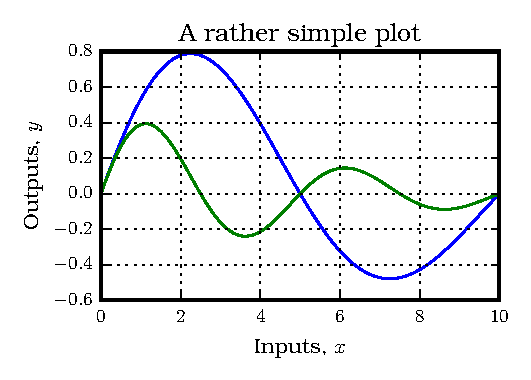
\includegraphics{simple_plot/mpl.pdf}
\end{center}

\subsection{Matplotlib + PGF backend}
\begin{center}
%% Creator: Matplotlib, PGF backend
%%
%% To include the figure in your LaTeX document, write
%%   \input{<filename>.pgf}
%%
%% Make sure the required packages are loaded in your preamble
%%   \usepackage{pgf}
%%
%% Figures using additional raster images can only be included by \input if
%% they are in the same directory as the main LaTeX file. For loading figures
%% from other directories you can use the `import` package
%%   \usepackage{import}
%% and then include the figures with
%%   \import{<path to file>}{<filename>.pgf}
%%
%% Matplotlib used the following preamble
%%   \usepackage{fontspec}
%%   \setmonofont{Courier}
%%
\begingroup%
\makeatletter%
\begin{pgfpicture}%
\pgfpathrectangle{\pgfpointorigin}{\pgfqpoint{3.543309in}{2.530935in}}%
\pgfusepath{use as bounding box, clip}%
\begin{pgfscope}%
\pgfsetbuttcap%
\pgfsetmiterjoin%
\definecolor{currentfill}{rgb}{1.000000,1.000000,1.000000}%
\pgfsetfillcolor{currentfill}%
\pgfsetlinewidth{0.000000pt}%
\definecolor{currentstroke}{rgb}{1.000000,1.000000,1.000000}%
\pgfsetstrokecolor{currentstroke}%
\pgfsetdash{}{0pt}%
\pgfpathmoveto{\pgfqpoint{0.000000in}{0.000000in}}%
\pgfpathlineto{\pgfqpoint{3.543309in}{0.000000in}}%
\pgfpathlineto{\pgfqpoint{3.543309in}{2.530935in}}%
\pgfpathlineto{\pgfqpoint{0.000000in}{2.530935in}}%
\pgfpathclose%
\pgfusepath{fill}%
\end{pgfscope}%
\begin{pgfscope}%
\pgfsetbuttcap%
\pgfsetmiterjoin%
\definecolor{currentfill}{rgb}{1.000000,1.000000,1.000000}%
\pgfsetfillcolor{currentfill}%
\pgfsetlinewidth{0.000000pt}%
\definecolor{currentstroke}{rgb}{0.000000,0.000000,0.000000}%
\pgfsetstrokecolor{currentstroke}%
\pgfsetstrokeopacity{0.000000}%
\pgfsetdash{}{0pt}%
\pgfpathmoveto{\pgfqpoint{0.672725in}{0.530800in}}%
\pgfpathlineto{\pgfqpoint{3.329313in}{0.530800in}}%
\pgfpathlineto{\pgfqpoint{3.329313in}{2.189698in}}%
\pgfpathlineto{\pgfqpoint{0.672725in}{2.189698in}}%
\pgfpathclose%
\pgfusepath{fill}%
\end{pgfscope}%
\begin{pgfscope}%
\pgfpathrectangle{\pgfqpoint{0.672725in}{0.530800in}}{\pgfqpoint{2.656588in}{1.658898in}} %
\pgfusepath{clip}%
\pgfsetrectcap%
\pgfsetroundjoin%
\pgfsetlinewidth{1.003750pt}%
\definecolor{currentstroke}{rgb}{0.000000,0.000000,1.000000}%
\pgfsetstrokecolor{currentstroke}%
\pgfsetdash{}{0pt}%
\pgfpathmoveto{\pgfqpoint{0.672725in}{1.241756in}}%
\pgfpathlineto{\pgfqpoint{0.699559in}{1.316154in}}%
\pgfpathlineto{\pgfqpoint{0.726394in}{1.388759in}}%
\pgfpathlineto{\pgfqpoint{0.753228in}{1.459312in}}%
\pgfpathlineto{\pgfqpoint{0.780062in}{1.527564in}}%
\pgfpathlineto{\pgfqpoint{0.806896in}{1.593283in}}%
\pgfpathlineto{\pgfqpoint{0.833730in}{1.656252in}}%
\pgfpathlineto{\pgfqpoint{0.860565in}{1.716266in}}%
\pgfpathlineto{\pgfqpoint{0.887399in}{1.773141in}}%
\pgfpathlineto{\pgfqpoint{0.914233in}{1.826707in}}%
\pgfpathlineto{\pgfqpoint{0.941067in}{1.876811in}}%
\pgfpathlineto{\pgfqpoint{0.967902in}{1.923317in}}%
\pgfpathlineto{\pgfqpoint{0.994736in}{1.966107in}}%
\pgfpathlineto{\pgfqpoint{1.021570in}{2.005081in}}%
\pgfpathlineto{\pgfqpoint{1.048404in}{2.040155in}}%
\pgfpathlineto{\pgfqpoint{1.075238in}{2.071265in}}%
\pgfpathlineto{\pgfqpoint{1.102073in}{2.098363in}}%
\pgfpathlineto{\pgfqpoint{1.128907in}{2.121417in}}%
\pgfpathlineto{\pgfqpoint{1.155741in}{2.140415in}}%
\pgfpathlineto{\pgfqpoint{1.182575in}{2.155360in}}%
\pgfpathlineto{\pgfqpoint{1.209410in}{2.166272in}}%
\pgfpathlineto{\pgfqpoint{1.236244in}{2.173187in}}%
\pgfpathlineto{\pgfqpoint{1.263078in}{2.176157in}}%
\pgfpathlineto{\pgfqpoint{1.289912in}{2.175249in}}%
\pgfpathlineto{\pgfqpoint{1.316746in}{2.170543in}}%
\pgfpathlineto{\pgfqpoint{1.343581in}{2.162135in}}%
\pgfpathlineto{\pgfqpoint{1.370415in}{2.150134in}}%
\pgfpathlineto{\pgfqpoint{1.397249in}{2.134660in}}%
\pgfpathlineto{\pgfqpoint{1.424083in}{2.115846in}}%
\pgfpathlineto{\pgfqpoint{1.450918in}{2.093836in}}%
\pgfpathlineto{\pgfqpoint{1.477752in}{2.068783in}}%
\pgfpathlineto{\pgfqpoint{1.504586in}{2.040851in}}%
\pgfpathlineto{\pgfqpoint{1.531420in}{2.010212in}}%
\pgfpathlineto{\pgfqpoint{1.558254in}{1.977044in}}%
\pgfpathlineto{\pgfqpoint{1.585089in}{1.941535in}}%
\pgfpathlineto{\pgfqpoint{1.611923in}{1.903876in}}%
\pgfpathlineto{\pgfqpoint{1.638757in}{1.864263in}}%
\pgfpathlineto{\pgfqpoint{1.665591in}{1.822899in}}%
\pgfpathlineto{\pgfqpoint{1.692426in}{1.779987in}}%
\pgfpathlineto{\pgfqpoint{1.719260in}{1.735733in}}%
\pgfpathlineto{\pgfqpoint{1.746094in}{1.690345in}}%
\pgfpathlineto{\pgfqpoint{1.772928in}{1.644031in}}%
\pgfpathlineto{\pgfqpoint{1.799763in}{1.597000in}}%
\pgfpathlineto{\pgfqpoint{1.826597in}{1.549457in}}%
\pgfpathlineto{\pgfqpoint{1.853431in}{1.501607in}}%
\pgfpathlineto{\pgfqpoint{1.880265in}{1.453652in}}%
\pgfpathlineto{\pgfqpoint{1.907099in}{1.405790in}}%
\pgfpathlineto{\pgfqpoint{1.933934in}{1.358215in}}%
\pgfpathlineto{\pgfqpoint{1.960768in}{1.311116in}}%
\pgfpathlineto{\pgfqpoint{1.987602in}{1.264675in}}%
\pgfpathlineto{\pgfqpoint{2.014436in}{1.219069in}}%
\pgfpathlineto{\pgfqpoint{2.041271in}{1.174467in}}%
\pgfpathlineto{\pgfqpoint{2.068105in}{1.131033in}}%
\pgfpathlineto{\pgfqpoint{2.094939in}{1.088920in}}%
\pgfpathlineto{\pgfqpoint{2.121773in}{1.048274in}}%
\pgfpathlineto{\pgfqpoint{2.148607in}{1.009232in}}%
\pgfpathlineto{\pgfqpoint{2.175442in}{0.971921in}}%
\pgfpathlineto{\pgfqpoint{2.202276in}{0.936459in}}%
\pgfpathlineto{\pgfqpoint{2.229110in}{0.902954in}}%
\pgfpathlineto{\pgfqpoint{2.255944in}{0.871503in}}%
\pgfpathlineto{\pgfqpoint{2.282779in}{0.842195in}}%
\pgfpathlineto{\pgfqpoint{2.309613in}{0.815107in}}%
\pgfpathlineto{\pgfqpoint{2.336447in}{0.790304in}}%
\pgfpathlineto{\pgfqpoint{2.363281in}{0.767842in}}%
\pgfpathlineto{\pgfqpoint{2.390115in}{0.747766in}}%
\pgfpathlineto{\pgfqpoint{2.416950in}{0.730111in}}%
\pgfpathlineto{\pgfqpoint{2.443784in}{0.714900in}}%
\pgfpathlineto{\pgfqpoint{2.470618in}{0.702146in}}%
\pgfpathlineto{\pgfqpoint{2.497452in}{0.691853in}}%
\pgfpathlineto{\pgfqpoint{2.524287in}{0.684014in}}%
\pgfpathlineto{\pgfqpoint{2.551121in}{0.678611in}}%
\pgfpathlineto{\pgfqpoint{2.577955in}{0.675618in}}%
\pgfpathlineto{\pgfqpoint{2.604789in}{0.674998in}}%
\pgfpathlineto{\pgfqpoint{2.631623in}{0.676707in}}%
\pgfpathlineto{\pgfqpoint{2.658458in}{0.680692in}}%
\pgfpathlineto{\pgfqpoint{2.685292in}{0.686890in}}%
\pgfpathlineto{\pgfqpoint{2.712126in}{0.695232in}}%
\pgfpathlineto{\pgfqpoint{2.738960in}{0.705641in}}%
\pgfpathlineto{\pgfqpoint{2.765795in}{0.718033in}}%
\pgfpathlineto{\pgfqpoint{2.792629in}{0.732317in}}%
\pgfpathlineto{\pgfqpoint{2.819463in}{0.748398in}}%
\pgfpathlineto{\pgfqpoint{2.846297in}{0.766174in}}%
\pgfpathlineto{\pgfqpoint{2.873131in}{0.785539in}}%
\pgfpathlineto{\pgfqpoint{2.899966in}{0.806380in}}%
\pgfpathlineto{\pgfqpoint{2.926800in}{0.828584in}}%
\pgfpathlineto{\pgfqpoint{2.953634in}{0.852033in}}%
\pgfpathlineto{\pgfqpoint{2.980468in}{0.876606in}}%
\pgfpathlineto{\pgfqpoint{3.007303in}{0.902180in}}%
\pgfpathlineto{\pgfqpoint{3.034137in}{0.928630in}}%
\pgfpathlineto{\pgfqpoint{3.060971in}{0.955831in}}%
\pgfpathlineto{\pgfqpoint{3.087805in}{0.983657in}}%
\pgfpathlineto{\pgfqpoint{3.114640in}{1.011981in}}%
\pgfpathlineto{\pgfqpoint{3.141474in}{1.040678in}}%
\pgfpathlineto{\pgfqpoint{3.168308in}{1.069622in}}%
\pgfpathlineto{\pgfqpoint{3.195142in}{1.098692in}}%
\pgfpathlineto{\pgfqpoint{3.221976in}{1.127765in}}%
\pgfpathlineto{\pgfqpoint{3.248811in}{1.156722in}}%
\pgfpathlineto{\pgfqpoint{3.275645in}{1.185447in}}%
\pgfpathlineto{\pgfqpoint{3.302479in}{1.213829in}}%
\pgfpathlineto{\pgfqpoint{3.329313in}{1.241756in}}%
\pgfusepath{stroke}%
\end{pgfscope}%
\begin{pgfscope}%
\pgfpathrectangle{\pgfqpoint{0.672725in}{0.530800in}}{\pgfqpoint{2.656588in}{1.658898in}} %
\pgfusepath{clip}%
\pgfsetrectcap%
\pgfsetroundjoin%
\pgfsetlinewidth{1.003750pt}%
\definecolor{currentstroke}{rgb}{0.000000,0.500000,0.000000}%
\pgfsetstrokecolor{currentstroke}%
\pgfsetdash{}{0pt}%
\pgfpathmoveto{\pgfqpoint{0.672725in}{1.241756in}}%
\pgfpathlineto{\pgfqpoint{0.699559in}{1.315258in}}%
\pgfpathlineto{\pgfqpoint{0.726394in}{1.384660in}}%
\pgfpathlineto{\pgfqpoint{0.753228in}{1.449004in}}%
\pgfpathlineto{\pgfqpoint{0.780062in}{1.507449in}}%
\pgfpathlineto{\pgfqpoint{0.806896in}{1.559284in}}%
\pgfpathlineto{\pgfqpoint{0.833730in}{1.603932in}}%
\pgfpathlineto{\pgfqpoint{0.860565in}{1.640956in}}%
\pgfpathlineto{\pgfqpoint{0.887399in}{1.670060in}}%
\pgfpathlineto{\pgfqpoint{0.914233in}{1.691086in}}%
\pgfpathlineto{\pgfqpoint{0.941067in}{1.704014in}}%
\pgfpathlineto{\pgfqpoint{0.967902in}{1.708957in}}%
\pgfpathlineto{\pgfqpoint{0.994736in}{1.706150in}}%
\pgfpathlineto{\pgfqpoint{1.021570in}{1.695945in}}%
\pgfpathlineto{\pgfqpoint{1.048404in}{1.678801in}}%
\pgfpathlineto{\pgfqpoint{1.075238in}{1.655270in}}%
\pgfpathlineto{\pgfqpoint{1.102073in}{1.625984in}}%
\pgfpathlineto{\pgfqpoint{1.128907in}{1.591646in}}%
\pgfpathlineto{\pgfqpoint{1.155741in}{1.553010in}}%
\pgfpathlineto{\pgfqpoint{1.182575in}{1.510872in}}%
\pgfpathlineto{\pgfqpoint{1.209410in}{1.466051in}}%
\pgfpathlineto{\pgfqpoint{1.236244in}{1.419378in}}%
\pgfpathlineto{\pgfqpoint{1.263078in}{1.371682in}}%
\pgfpathlineto{\pgfqpoint{1.289912in}{1.323773in}}%
\pgfpathlineto{\pgfqpoint{1.316746in}{1.276436in}}%
\pgfpathlineto{\pgfqpoint{1.343581in}{1.230413in}}%
\pgfpathlineto{\pgfqpoint{1.370415in}{1.186395in}}%
\pgfpathlineto{\pgfqpoint{1.397249in}{1.145015in}}%
\pgfpathlineto{\pgfqpoint{1.424083in}{1.106839in}}%
\pgfpathlineto{\pgfqpoint{1.450918in}{1.072355in}}%
\pgfpathlineto{\pgfqpoint{1.477752in}{1.041976in}}%
\pgfpathlineto{\pgfqpoint{1.504586in}{1.016030in}}%
\pgfpathlineto{\pgfqpoint{1.531420in}{0.994761in}}%
\pgfpathlineto{\pgfqpoint{1.558254in}{0.978328in}}%
\pgfpathlineto{\pgfqpoint{1.585089in}{0.966805in}}%
\pgfpathlineto{\pgfqpoint{1.611923in}{0.960184in}}%
\pgfpathlineto{\pgfqpoint{1.638757in}{0.958377in}}%
\pgfpathlineto{\pgfqpoint{1.665591in}{0.961224in}}%
\pgfpathlineto{\pgfqpoint{1.692426in}{0.968494in}}%
\pgfpathlineto{\pgfqpoint{1.719260in}{0.979895in}}%
\pgfpathlineto{\pgfqpoint{1.746094in}{0.995077in}}%
\pgfpathlineto{\pgfqpoint{1.772928in}{1.013647in}}%
\pgfpathlineto{\pgfqpoint{1.799763in}{1.035170in}}%
\pgfpathlineto{\pgfqpoint{1.826597in}{1.059181in}}%
\pgfpathlineto{\pgfqpoint{1.853431in}{1.085193in}}%
\pgfpathlineto{\pgfqpoint{1.880265in}{1.112707in}}%
\pgfpathlineto{\pgfqpoint{1.907099in}{1.141217in}}%
\pgfpathlineto{\pgfqpoint{1.933934in}{1.170224in}}%
\pgfpathlineto{\pgfqpoint{1.960768in}{1.199239in}}%
\pgfpathlineto{\pgfqpoint{1.987602in}{1.227793in}}%
\pgfpathlineto{\pgfqpoint{2.014436in}{1.255441in}}%
\pgfpathlineto{\pgfqpoint{2.041271in}{1.281774in}}%
\pgfpathlineto{\pgfqpoint{2.068105in}{1.306416in}}%
\pgfpathlineto{\pgfqpoint{2.094939in}{1.329038in}}%
\pgfpathlineto{\pgfqpoint{2.121773in}{1.349352in}}%
\pgfpathlineto{\pgfqpoint{2.148607in}{1.367122in}}%
\pgfpathlineto{\pgfqpoint{2.175442in}{1.382162in}}%
\pgfpathlineto{\pgfqpoint{2.202276in}{1.394336in}}%
\pgfpathlineto{\pgfqpoint{2.229110in}{1.403561in}}%
\pgfpathlineto{\pgfqpoint{2.255944in}{1.409804in}}%
\pgfpathlineto{\pgfqpoint{2.282779in}{1.413084in}}%
\pgfpathlineto{\pgfqpoint{2.309613in}{1.413463in}}%
\pgfpathlineto{\pgfqpoint{2.336447in}{1.411051in}}%
\pgfpathlineto{\pgfqpoint{2.363281in}{1.405997in}}%
\pgfpathlineto{\pgfqpoint{2.390115in}{1.398488in}}%
\pgfpathlineto{\pgfqpoint{2.416950in}{1.388742in}}%
\pgfpathlineto{\pgfqpoint{2.443784in}{1.377005in}}%
\pgfpathlineto{\pgfqpoint{2.470618in}{1.363546in}}%
\pgfpathlineto{\pgfqpoint{2.497452in}{1.348652in}}%
\pgfpathlineto{\pgfqpoint{2.524287in}{1.332618in}}%
\pgfpathlineto{\pgfqpoint{2.551121in}{1.315751in}}%
\pgfpathlineto{\pgfqpoint{2.577955in}{1.298355in}}%
\pgfpathlineto{\pgfqpoint{2.604789in}{1.280732in}}%
\pgfpathlineto{\pgfqpoint{2.631623in}{1.263178in}}%
\pgfpathlineto{\pgfqpoint{2.658458in}{1.245972in}}%
\pgfpathlineto{\pgfqpoint{2.685292in}{1.229379in}}%
\pgfpathlineto{\pgfqpoint{2.712126in}{1.213644in}}%
\pgfpathlineto{\pgfqpoint{2.738960in}{1.198986in}}%
\pgfpathlineto{\pgfqpoint{2.765795in}{1.185600in}}%
\pgfpathlineto{\pgfqpoint{2.792629in}{1.173652in}}%
\pgfpathlineto{\pgfqpoint{2.819463in}{1.163279in}}%
\pgfpathlineto{\pgfqpoint{2.846297in}{1.154585in}}%
\pgfpathlineto{\pgfqpoint{2.873131in}{1.147644in}}%
\pgfpathlineto{\pgfqpoint{2.899966in}{1.142501in}}%
\pgfpathlineto{\pgfqpoint{2.926800in}{1.139165in}}%
\pgfpathlineto{\pgfqpoint{2.953634in}{1.137621in}}%
\pgfpathlineto{\pgfqpoint{2.980468in}{1.137821in}}%
\pgfpathlineto{\pgfqpoint{3.007303in}{1.139694in}}%
\pgfpathlineto{\pgfqpoint{3.034137in}{1.143143in}}%
\pgfpathlineto{\pgfqpoint{3.060971in}{1.148050in}}%
\pgfpathlineto{\pgfqpoint{3.087805in}{1.154278in}}%
\pgfpathlineto{\pgfqpoint{3.114640in}{1.161673in}}%
\pgfpathlineto{\pgfqpoint{3.141474in}{1.170071in}}%
\pgfpathlineto{\pgfqpoint{3.168308in}{1.179295in}}%
\pgfpathlineto{\pgfqpoint{3.195142in}{1.189163in}}%
\pgfpathlineto{\pgfqpoint{3.221976in}{1.199492in}}%
\pgfpathlineto{\pgfqpoint{3.248811in}{1.210094in}}%
\pgfpathlineto{\pgfqpoint{3.275645in}{1.220789in}}%
\pgfpathlineto{\pgfqpoint{3.302479in}{1.231399in}}%
\pgfpathlineto{\pgfqpoint{3.329313in}{1.241756in}}%
\pgfusepath{stroke}%
\end{pgfscope}%
\begin{pgfscope}%
\pgfsetrectcap%
\pgfsetmiterjoin%
\pgfsetlinewidth{1.505625pt}%
\definecolor{currentstroke}{rgb}{0.000000,0.000000,0.000000}%
\pgfsetstrokecolor{currentstroke}%
\pgfsetdash{}{0pt}%
\pgfpathmoveto{\pgfqpoint{0.672725in}{2.189698in}}%
\pgfpathlineto{\pgfqpoint{3.329313in}{2.189698in}}%
\pgfusepath{stroke}%
\end{pgfscope}%
\begin{pgfscope}%
\pgfsetrectcap%
\pgfsetmiterjoin%
\pgfsetlinewidth{1.505625pt}%
\definecolor{currentstroke}{rgb}{0.000000,0.000000,0.000000}%
\pgfsetstrokecolor{currentstroke}%
\pgfsetdash{}{0pt}%
\pgfpathmoveto{\pgfqpoint{3.329313in}{0.530800in}}%
\pgfpathlineto{\pgfqpoint{3.329313in}{2.189698in}}%
\pgfusepath{stroke}%
\end{pgfscope}%
\begin{pgfscope}%
\pgfsetrectcap%
\pgfsetmiterjoin%
\pgfsetlinewidth{1.505625pt}%
\definecolor{currentstroke}{rgb}{0.000000,0.000000,0.000000}%
\pgfsetstrokecolor{currentstroke}%
\pgfsetdash{}{0pt}%
\pgfpathmoveto{\pgfqpoint{0.672725in}{0.530800in}}%
\pgfpathlineto{\pgfqpoint{3.329313in}{0.530800in}}%
\pgfusepath{stroke}%
\end{pgfscope}%
\begin{pgfscope}%
\pgfsetrectcap%
\pgfsetmiterjoin%
\pgfsetlinewidth{1.505625pt}%
\definecolor{currentstroke}{rgb}{0.000000,0.000000,0.000000}%
\pgfsetstrokecolor{currentstroke}%
\pgfsetdash{}{0pt}%
\pgfpathmoveto{\pgfqpoint{0.672725in}{0.530800in}}%
\pgfpathlineto{\pgfqpoint{0.672725in}{2.189698in}}%
\pgfusepath{stroke}%
\end{pgfscope}%
\begin{pgfscope}%
\pgfpathrectangle{\pgfqpoint{0.672725in}{0.530800in}}{\pgfqpoint{2.656588in}{1.658898in}} %
\pgfusepath{clip}%
\pgfsetbuttcap%
\pgfsetroundjoin%
\pgfsetlinewidth{0.501875pt}%
\definecolor{currentstroke}{rgb}{0.000000,0.000000,0.000000}%
\pgfsetstrokecolor{currentstroke}%
\pgfsetdash{{1.000000pt}{3.000000pt}}{0.000000pt}%
\pgfpathmoveto{\pgfqpoint{0.672725in}{0.530800in}}%
\pgfpathlineto{\pgfqpoint{0.672725in}{2.189698in}}%
\pgfusepath{stroke}%
\end{pgfscope}%
\begin{pgfscope}%
\pgfsetbuttcap%
\pgfsetroundjoin%
\definecolor{currentfill}{rgb}{0.000000,0.000000,0.000000}%
\pgfsetfillcolor{currentfill}%
\pgfsetlinewidth{0.501875pt}%
\definecolor{currentstroke}{rgb}{0.000000,0.000000,0.000000}%
\pgfsetstrokecolor{currentstroke}%
\pgfsetdash{}{0pt}%
\pgfsys@defobject{currentmarker}{\pgfqpoint{0.000000in}{0.000000in}}{\pgfqpoint{0.000000in}{0.055556in}}{%
\pgfpathmoveto{\pgfqpoint{0.000000in}{0.000000in}}%
\pgfpathlineto{\pgfqpoint{0.000000in}{0.055556in}}%
\pgfusepath{stroke,fill}%
}%
\begin{pgfscope}%
\pgfsys@transformshift{0.672725in}{0.530800in}%
\pgfsys@useobject{currentmarker}{}%
\end{pgfscope}%
\end{pgfscope}%
\begin{pgfscope}%
\pgfsetbuttcap%
\pgfsetroundjoin%
\definecolor{currentfill}{rgb}{0.000000,0.000000,0.000000}%
\pgfsetfillcolor{currentfill}%
\pgfsetlinewidth{0.501875pt}%
\definecolor{currentstroke}{rgb}{0.000000,0.000000,0.000000}%
\pgfsetstrokecolor{currentstroke}%
\pgfsetdash{}{0pt}%
\pgfsys@defobject{currentmarker}{\pgfqpoint{0.000000in}{-0.055556in}}{\pgfqpoint{0.000000in}{0.000000in}}{%
\pgfpathmoveto{\pgfqpoint{0.000000in}{0.000000in}}%
\pgfpathlineto{\pgfqpoint{0.000000in}{-0.055556in}}%
\pgfusepath{stroke,fill}%
}%
\begin{pgfscope}%
\pgfsys@transformshift{0.672725in}{2.189698in}%
\pgfsys@useobject{currentmarker}{}%
\end{pgfscope}%
\end{pgfscope}%
\begin{pgfscope}%
\pgftext[x=0.672725in,y=0.475245in,,top]{\rmfamily\fontsize{9.000000}{10.800000}\selectfont \(\displaystyle 0\)}%
\end{pgfscope}%
\begin{pgfscope}%
\pgfpathrectangle{\pgfqpoint{0.672725in}{0.530800in}}{\pgfqpoint{2.656588in}{1.658898in}} %
\pgfusepath{clip}%
\pgfsetbuttcap%
\pgfsetroundjoin%
\pgfsetlinewidth{0.501875pt}%
\definecolor{currentstroke}{rgb}{0.000000,0.000000,0.000000}%
\pgfsetstrokecolor{currentstroke}%
\pgfsetdash{{1.000000pt}{3.000000pt}}{0.000000pt}%
\pgfpathmoveto{\pgfqpoint{1.204043in}{0.530800in}}%
\pgfpathlineto{\pgfqpoint{1.204043in}{2.189698in}}%
\pgfusepath{stroke}%
\end{pgfscope}%
\begin{pgfscope}%
\pgfsetbuttcap%
\pgfsetroundjoin%
\definecolor{currentfill}{rgb}{0.000000,0.000000,0.000000}%
\pgfsetfillcolor{currentfill}%
\pgfsetlinewidth{0.501875pt}%
\definecolor{currentstroke}{rgb}{0.000000,0.000000,0.000000}%
\pgfsetstrokecolor{currentstroke}%
\pgfsetdash{}{0pt}%
\pgfsys@defobject{currentmarker}{\pgfqpoint{0.000000in}{0.000000in}}{\pgfqpoint{0.000000in}{0.055556in}}{%
\pgfpathmoveto{\pgfqpoint{0.000000in}{0.000000in}}%
\pgfpathlineto{\pgfqpoint{0.000000in}{0.055556in}}%
\pgfusepath{stroke,fill}%
}%
\begin{pgfscope}%
\pgfsys@transformshift{1.204043in}{0.530800in}%
\pgfsys@useobject{currentmarker}{}%
\end{pgfscope}%
\end{pgfscope}%
\begin{pgfscope}%
\pgfsetbuttcap%
\pgfsetroundjoin%
\definecolor{currentfill}{rgb}{0.000000,0.000000,0.000000}%
\pgfsetfillcolor{currentfill}%
\pgfsetlinewidth{0.501875pt}%
\definecolor{currentstroke}{rgb}{0.000000,0.000000,0.000000}%
\pgfsetstrokecolor{currentstroke}%
\pgfsetdash{}{0pt}%
\pgfsys@defobject{currentmarker}{\pgfqpoint{0.000000in}{-0.055556in}}{\pgfqpoint{0.000000in}{0.000000in}}{%
\pgfpathmoveto{\pgfqpoint{0.000000in}{0.000000in}}%
\pgfpathlineto{\pgfqpoint{0.000000in}{-0.055556in}}%
\pgfusepath{stroke,fill}%
}%
\begin{pgfscope}%
\pgfsys@transformshift{1.204043in}{2.189698in}%
\pgfsys@useobject{currentmarker}{}%
\end{pgfscope}%
\end{pgfscope}%
\begin{pgfscope}%
\pgftext[x=1.204043in,y=0.475245in,,top]{\rmfamily\fontsize{9.000000}{10.800000}\selectfont \(\displaystyle 2\)}%
\end{pgfscope}%
\begin{pgfscope}%
\pgfpathrectangle{\pgfqpoint{0.672725in}{0.530800in}}{\pgfqpoint{2.656588in}{1.658898in}} %
\pgfusepath{clip}%
\pgfsetbuttcap%
\pgfsetroundjoin%
\pgfsetlinewidth{0.501875pt}%
\definecolor{currentstroke}{rgb}{0.000000,0.000000,0.000000}%
\pgfsetstrokecolor{currentstroke}%
\pgfsetdash{{1.000000pt}{3.000000pt}}{0.000000pt}%
\pgfpathmoveto{\pgfqpoint{1.735360in}{0.530800in}}%
\pgfpathlineto{\pgfqpoint{1.735360in}{2.189698in}}%
\pgfusepath{stroke}%
\end{pgfscope}%
\begin{pgfscope}%
\pgfsetbuttcap%
\pgfsetroundjoin%
\definecolor{currentfill}{rgb}{0.000000,0.000000,0.000000}%
\pgfsetfillcolor{currentfill}%
\pgfsetlinewidth{0.501875pt}%
\definecolor{currentstroke}{rgb}{0.000000,0.000000,0.000000}%
\pgfsetstrokecolor{currentstroke}%
\pgfsetdash{}{0pt}%
\pgfsys@defobject{currentmarker}{\pgfqpoint{0.000000in}{0.000000in}}{\pgfqpoint{0.000000in}{0.055556in}}{%
\pgfpathmoveto{\pgfqpoint{0.000000in}{0.000000in}}%
\pgfpathlineto{\pgfqpoint{0.000000in}{0.055556in}}%
\pgfusepath{stroke,fill}%
}%
\begin{pgfscope}%
\pgfsys@transformshift{1.735360in}{0.530800in}%
\pgfsys@useobject{currentmarker}{}%
\end{pgfscope}%
\end{pgfscope}%
\begin{pgfscope}%
\pgfsetbuttcap%
\pgfsetroundjoin%
\definecolor{currentfill}{rgb}{0.000000,0.000000,0.000000}%
\pgfsetfillcolor{currentfill}%
\pgfsetlinewidth{0.501875pt}%
\definecolor{currentstroke}{rgb}{0.000000,0.000000,0.000000}%
\pgfsetstrokecolor{currentstroke}%
\pgfsetdash{}{0pt}%
\pgfsys@defobject{currentmarker}{\pgfqpoint{0.000000in}{-0.055556in}}{\pgfqpoint{0.000000in}{0.000000in}}{%
\pgfpathmoveto{\pgfqpoint{0.000000in}{0.000000in}}%
\pgfpathlineto{\pgfqpoint{0.000000in}{-0.055556in}}%
\pgfusepath{stroke,fill}%
}%
\begin{pgfscope}%
\pgfsys@transformshift{1.735360in}{2.189698in}%
\pgfsys@useobject{currentmarker}{}%
\end{pgfscope}%
\end{pgfscope}%
\begin{pgfscope}%
\pgftext[x=1.735360in,y=0.475245in,,top]{\rmfamily\fontsize{9.000000}{10.800000}\selectfont \(\displaystyle 4\)}%
\end{pgfscope}%
\begin{pgfscope}%
\pgfpathrectangle{\pgfqpoint{0.672725in}{0.530800in}}{\pgfqpoint{2.656588in}{1.658898in}} %
\pgfusepath{clip}%
\pgfsetbuttcap%
\pgfsetroundjoin%
\pgfsetlinewidth{0.501875pt}%
\definecolor{currentstroke}{rgb}{0.000000,0.000000,0.000000}%
\pgfsetstrokecolor{currentstroke}%
\pgfsetdash{{1.000000pt}{3.000000pt}}{0.000000pt}%
\pgfpathmoveto{\pgfqpoint{2.266678in}{0.530800in}}%
\pgfpathlineto{\pgfqpoint{2.266678in}{2.189698in}}%
\pgfusepath{stroke}%
\end{pgfscope}%
\begin{pgfscope}%
\pgfsetbuttcap%
\pgfsetroundjoin%
\definecolor{currentfill}{rgb}{0.000000,0.000000,0.000000}%
\pgfsetfillcolor{currentfill}%
\pgfsetlinewidth{0.501875pt}%
\definecolor{currentstroke}{rgb}{0.000000,0.000000,0.000000}%
\pgfsetstrokecolor{currentstroke}%
\pgfsetdash{}{0pt}%
\pgfsys@defobject{currentmarker}{\pgfqpoint{0.000000in}{0.000000in}}{\pgfqpoint{0.000000in}{0.055556in}}{%
\pgfpathmoveto{\pgfqpoint{0.000000in}{0.000000in}}%
\pgfpathlineto{\pgfqpoint{0.000000in}{0.055556in}}%
\pgfusepath{stroke,fill}%
}%
\begin{pgfscope}%
\pgfsys@transformshift{2.266678in}{0.530800in}%
\pgfsys@useobject{currentmarker}{}%
\end{pgfscope}%
\end{pgfscope}%
\begin{pgfscope}%
\pgfsetbuttcap%
\pgfsetroundjoin%
\definecolor{currentfill}{rgb}{0.000000,0.000000,0.000000}%
\pgfsetfillcolor{currentfill}%
\pgfsetlinewidth{0.501875pt}%
\definecolor{currentstroke}{rgb}{0.000000,0.000000,0.000000}%
\pgfsetstrokecolor{currentstroke}%
\pgfsetdash{}{0pt}%
\pgfsys@defobject{currentmarker}{\pgfqpoint{0.000000in}{-0.055556in}}{\pgfqpoint{0.000000in}{0.000000in}}{%
\pgfpathmoveto{\pgfqpoint{0.000000in}{0.000000in}}%
\pgfpathlineto{\pgfqpoint{0.000000in}{-0.055556in}}%
\pgfusepath{stroke,fill}%
}%
\begin{pgfscope}%
\pgfsys@transformshift{2.266678in}{2.189698in}%
\pgfsys@useobject{currentmarker}{}%
\end{pgfscope}%
\end{pgfscope}%
\begin{pgfscope}%
\pgftext[x=2.266678in,y=0.475245in,,top]{\rmfamily\fontsize{9.000000}{10.800000}\selectfont \(\displaystyle 6\)}%
\end{pgfscope}%
\begin{pgfscope}%
\pgfpathrectangle{\pgfqpoint{0.672725in}{0.530800in}}{\pgfqpoint{2.656588in}{1.658898in}} %
\pgfusepath{clip}%
\pgfsetbuttcap%
\pgfsetroundjoin%
\pgfsetlinewidth{0.501875pt}%
\definecolor{currentstroke}{rgb}{0.000000,0.000000,0.000000}%
\pgfsetstrokecolor{currentstroke}%
\pgfsetdash{{1.000000pt}{3.000000pt}}{0.000000pt}%
\pgfpathmoveto{\pgfqpoint{2.797996in}{0.530800in}}%
\pgfpathlineto{\pgfqpoint{2.797996in}{2.189698in}}%
\pgfusepath{stroke}%
\end{pgfscope}%
\begin{pgfscope}%
\pgfsetbuttcap%
\pgfsetroundjoin%
\definecolor{currentfill}{rgb}{0.000000,0.000000,0.000000}%
\pgfsetfillcolor{currentfill}%
\pgfsetlinewidth{0.501875pt}%
\definecolor{currentstroke}{rgb}{0.000000,0.000000,0.000000}%
\pgfsetstrokecolor{currentstroke}%
\pgfsetdash{}{0pt}%
\pgfsys@defobject{currentmarker}{\pgfqpoint{0.000000in}{0.000000in}}{\pgfqpoint{0.000000in}{0.055556in}}{%
\pgfpathmoveto{\pgfqpoint{0.000000in}{0.000000in}}%
\pgfpathlineto{\pgfqpoint{0.000000in}{0.055556in}}%
\pgfusepath{stroke,fill}%
}%
\begin{pgfscope}%
\pgfsys@transformshift{2.797996in}{0.530800in}%
\pgfsys@useobject{currentmarker}{}%
\end{pgfscope}%
\end{pgfscope}%
\begin{pgfscope}%
\pgfsetbuttcap%
\pgfsetroundjoin%
\definecolor{currentfill}{rgb}{0.000000,0.000000,0.000000}%
\pgfsetfillcolor{currentfill}%
\pgfsetlinewidth{0.501875pt}%
\definecolor{currentstroke}{rgb}{0.000000,0.000000,0.000000}%
\pgfsetstrokecolor{currentstroke}%
\pgfsetdash{}{0pt}%
\pgfsys@defobject{currentmarker}{\pgfqpoint{0.000000in}{-0.055556in}}{\pgfqpoint{0.000000in}{0.000000in}}{%
\pgfpathmoveto{\pgfqpoint{0.000000in}{0.000000in}}%
\pgfpathlineto{\pgfqpoint{0.000000in}{-0.055556in}}%
\pgfusepath{stroke,fill}%
}%
\begin{pgfscope}%
\pgfsys@transformshift{2.797996in}{2.189698in}%
\pgfsys@useobject{currentmarker}{}%
\end{pgfscope}%
\end{pgfscope}%
\begin{pgfscope}%
\pgftext[x=2.797996in,y=0.475245in,,top]{\rmfamily\fontsize{9.000000}{10.800000}\selectfont \(\displaystyle 8\)}%
\end{pgfscope}%
\begin{pgfscope}%
\pgfpathrectangle{\pgfqpoint{0.672725in}{0.530800in}}{\pgfqpoint{2.656588in}{1.658898in}} %
\pgfusepath{clip}%
\pgfsetbuttcap%
\pgfsetroundjoin%
\pgfsetlinewidth{0.501875pt}%
\definecolor{currentstroke}{rgb}{0.000000,0.000000,0.000000}%
\pgfsetstrokecolor{currentstroke}%
\pgfsetdash{{1.000000pt}{3.000000pt}}{0.000000pt}%
\pgfpathmoveto{\pgfqpoint{3.329313in}{0.530800in}}%
\pgfpathlineto{\pgfqpoint{3.329313in}{2.189698in}}%
\pgfusepath{stroke}%
\end{pgfscope}%
\begin{pgfscope}%
\pgfsetbuttcap%
\pgfsetroundjoin%
\definecolor{currentfill}{rgb}{0.000000,0.000000,0.000000}%
\pgfsetfillcolor{currentfill}%
\pgfsetlinewidth{0.501875pt}%
\definecolor{currentstroke}{rgb}{0.000000,0.000000,0.000000}%
\pgfsetstrokecolor{currentstroke}%
\pgfsetdash{}{0pt}%
\pgfsys@defobject{currentmarker}{\pgfqpoint{0.000000in}{0.000000in}}{\pgfqpoint{0.000000in}{0.055556in}}{%
\pgfpathmoveto{\pgfqpoint{0.000000in}{0.000000in}}%
\pgfpathlineto{\pgfqpoint{0.000000in}{0.055556in}}%
\pgfusepath{stroke,fill}%
}%
\begin{pgfscope}%
\pgfsys@transformshift{3.329313in}{0.530800in}%
\pgfsys@useobject{currentmarker}{}%
\end{pgfscope}%
\end{pgfscope}%
\begin{pgfscope}%
\pgfsetbuttcap%
\pgfsetroundjoin%
\definecolor{currentfill}{rgb}{0.000000,0.000000,0.000000}%
\pgfsetfillcolor{currentfill}%
\pgfsetlinewidth{0.501875pt}%
\definecolor{currentstroke}{rgb}{0.000000,0.000000,0.000000}%
\pgfsetstrokecolor{currentstroke}%
\pgfsetdash{}{0pt}%
\pgfsys@defobject{currentmarker}{\pgfqpoint{0.000000in}{-0.055556in}}{\pgfqpoint{0.000000in}{0.000000in}}{%
\pgfpathmoveto{\pgfqpoint{0.000000in}{0.000000in}}%
\pgfpathlineto{\pgfqpoint{0.000000in}{-0.055556in}}%
\pgfusepath{stroke,fill}%
}%
\begin{pgfscope}%
\pgfsys@transformshift{3.329313in}{2.189698in}%
\pgfsys@useobject{currentmarker}{}%
\end{pgfscope}%
\end{pgfscope}%
\begin{pgfscope}%
\pgftext[x=3.329313in,y=0.475245in,,top]{\rmfamily\fontsize{9.000000}{10.800000}\selectfont \(\displaystyle 10\)}%
\end{pgfscope}%
\begin{pgfscope}%
\pgftext[x=2.001019in,y=0.294800in,,top]{\rmfamily\fontsize{10.000000}{12.000000}\selectfont Inputs,  \(\displaystyle x\)}%
\end{pgfscope}%
\begin{pgfscope}%
\pgfpathrectangle{\pgfqpoint{0.672725in}{0.530800in}}{\pgfqpoint{2.656588in}{1.658898in}} %
\pgfusepath{clip}%
\pgfsetbuttcap%
\pgfsetroundjoin%
\pgfsetlinewidth{0.501875pt}%
\definecolor{currentstroke}{rgb}{0.000000,0.000000,0.000000}%
\pgfsetstrokecolor{currentstroke}%
\pgfsetdash{{1.000000pt}{3.000000pt}}{0.000000pt}%
\pgfpathmoveto{\pgfqpoint{0.672725in}{0.530800in}}%
\pgfpathlineto{\pgfqpoint{3.329313in}{0.530800in}}%
\pgfusepath{stroke}%
\end{pgfscope}%
\begin{pgfscope}%
\pgfsetbuttcap%
\pgfsetroundjoin%
\definecolor{currentfill}{rgb}{0.000000,0.000000,0.000000}%
\pgfsetfillcolor{currentfill}%
\pgfsetlinewidth{0.501875pt}%
\definecolor{currentstroke}{rgb}{0.000000,0.000000,0.000000}%
\pgfsetstrokecolor{currentstroke}%
\pgfsetdash{}{0pt}%
\pgfsys@defobject{currentmarker}{\pgfqpoint{0.000000in}{0.000000in}}{\pgfqpoint{0.055556in}{0.000000in}}{%
\pgfpathmoveto{\pgfqpoint{0.000000in}{0.000000in}}%
\pgfpathlineto{\pgfqpoint{0.055556in}{0.000000in}}%
\pgfusepath{stroke,fill}%
}%
\begin{pgfscope}%
\pgfsys@transformshift{0.672725in}{0.530800in}%
\pgfsys@useobject{currentmarker}{}%
\end{pgfscope}%
\end{pgfscope}%
\begin{pgfscope}%
\pgfsetbuttcap%
\pgfsetroundjoin%
\definecolor{currentfill}{rgb}{0.000000,0.000000,0.000000}%
\pgfsetfillcolor{currentfill}%
\pgfsetlinewidth{0.501875pt}%
\definecolor{currentstroke}{rgb}{0.000000,0.000000,0.000000}%
\pgfsetstrokecolor{currentstroke}%
\pgfsetdash{}{0pt}%
\pgfsys@defobject{currentmarker}{\pgfqpoint{-0.055556in}{0.000000in}}{\pgfqpoint{0.000000in}{0.000000in}}{%
\pgfpathmoveto{\pgfqpoint{0.000000in}{0.000000in}}%
\pgfpathlineto{\pgfqpoint{-0.055556in}{0.000000in}}%
\pgfusepath{stroke,fill}%
}%
\begin{pgfscope}%
\pgfsys@transformshift{3.329313in}{0.530800in}%
\pgfsys@useobject{currentmarker}{}%
\end{pgfscope}%
\end{pgfscope}%
\begin{pgfscope}%
\pgftext[x=0.617170in,y=0.530800in,right,]{\rmfamily\fontsize{9.000000}{10.800000}\selectfont \(\displaystyle -0.6\)}%
\end{pgfscope}%
\begin{pgfscope}%
\pgfpathrectangle{\pgfqpoint{0.672725in}{0.530800in}}{\pgfqpoint{2.656588in}{1.658898in}} %
\pgfusepath{clip}%
\pgfsetbuttcap%
\pgfsetroundjoin%
\pgfsetlinewidth{0.501875pt}%
\definecolor{currentstroke}{rgb}{0.000000,0.000000,0.000000}%
\pgfsetstrokecolor{currentstroke}%
\pgfsetdash{{1.000000pt}{3.000000pt}}{0.000000pt}%
\pgfpathmoveto{\pgfqpoint{0.672725in}{0.767786in}}%
\pgfpathlineto{\pgfqpoint{3.329313in}{0.767786in}}%
\pgfusepath{stroke}%
\end{pgfscope}%
\begin{pgfscope}%
\pgfsetbuttcap%
\pgfsetroundjoin%
\definecolor{currentfill}{rgb}{0.000000,0.000000,0.000000}%
\pgfsetfillcolor{currentfill}%
\pgfsetlinewidth{0.501875pt}%
\definecolor{currentstroke}{rgb}{0.000000,0.000000,0.000000}%
\pgfsetstrokecolor{currentstroke}%
\pgfsetdash{}{0pt}%
\pgfsys@defobject{currentmarker}{\pgfqpoint{0.000000in}{0.000000in}}{\pgfqpoint{0.055556in}{0.000000in}}{%
\pgfpathmoveto{\pgfqpoint{0.000000in}{0.000000in}}%
\pgfpathlineto{\pgfqpoint{0.055556in}{0.000000in}}%
\pgfusepath{stroke,fill}%
}%
\begin{pgfscope}%
\pgfsys@transformshift{0.672725in}{0.767786in}%
\pgfsys@useobject{currentmarker}{}%
\end{pgfscope}%
\end{pgfscope}%
\begin{pgfscope}%
\pgfsetbuttcap%
\pgfsetroundjoin%
\definecolor{currentfill}{rgb}{0.000000,0.000000,0.000000}%
\pgfsetfillcolor{currentfill}%
\pgfsetlinewidth{0.501875pt}%
\definecolor{currentstroke}{rgb}{0.000000,0.000000,0.000000}%
\pgfsetstrokecolor{currentstroke}%
\pgfsetdash{}{0pt}%
\pgfsys@defobject{currentmarker}{\pgfqpoint{-0.055556in}{0.000000in}}{\pgfqpoint{0.000000in}{0.000000in}}{%
\pgfpathmoveto{\pgfqpoint{0.000000in}{0.000000in}}%
\pgfpathlineto{\pgfqpoint{-0.055556in}{0.000000in}}%
\pgfusepath{stroke,fill}%
}%
\begin{pgfscope}%
\pgfsys@transformshift{3.329313in}{0.767786in}%
\pgfsys@useobject{currentmarker}{}%
\end{pgfscope}%
\end{pgfscope}%
\begin{pgfscope}%
\pgftext[x=0.617170in,y=0.767786in,right,]{\rmfamily\fontsize{9.000000}{10.800000}\selectfont \(\displaystyle -0.4\)}%
\end{pgfscope}%
\begin{pgfscope}%
\pgfpathrectangle{\pgfqpoint{0.672725in}{0.530800in}}{\pgfqpoint{2.656588in}{1.658898in}} %
\pgfusepath{clip}%
\pgfsetbuttcap%
\pgfsetroundjoin%
\pgfsetlinewidth{0.501875pt}%
\definecolor{currentstroke}{rgb}{0.000000,0.000000,0.000000}%
\pgfsetstrokecolor{currentstroke}%
\pgfsetdash{{1.000000pt}{3.000000pt}}{0.000000pt}%
\pgfpathmoveto{\pgfqpoint{0.672725in}{1.004771in}}%
\pgfpathlineto{\pgfqpoint{3.329313in}{1.004771in}}%
\pgfusepath{stroke}%
\end{pgfscope}%
\begin{pgfscope}%
\pgfsetbuttcap%
\pgfsetroundjoin%
\definecolor{currentfill}{rgb}{0.000000,0.000000,0.000000}%
\pgfsetfillcolor{currentfill}%
\pgfsetlinewidth{0.501875pt}%
\definecolor{currentstroke}{rgb}{0.000000,0.000000,0.000000}%
\pgfsetstrokecolor{currentstroke}%
\pgfsetdash{}{0pt}%
\pgfsys@defobject{currentmarker}{\pgfqpoint{0.000000in}{0.000000in}}{\pgfqpoint{0.055556in}{0.000000in}}{%
\pgfpathmoveto{\pgfqpoint{0.000000in}{0.000000in}}%
\pgfpathlineto{\pgfqpoint{0.055556in}{0.000000in}}%
\pgfusepath{stroke,fill}%
}%
\begin{pgfscope}%
\pgfsys@transformshift{0.672725in}{1.004771in}%
\pgfsys@useobject{currentmarker}{}%
\end{pgfscope}%
\end{pgfscope}%
\begin{pgfscope}%
\pgfsetbuttcap%
\pgfsetroundjoin%
\definecolor{currentfill}{rgb}{0.000000,0.000000,0.000000}%
\pgfsetfillcolor{currentfill}%
\pgfsetlinewidth{0.501875pt}%
\definecolor{currentstroke}{rgb}{0.000000,0.000000,0.000000}%
\pgfsetstrokecolor{currentstroke}%
\pgfsetdash{}{0pt}%
\pgfsys@defobject{currentmarker}{\pgfqpoint{-0.055556in}{0.000000in}}{\pgfqpoint{0.000000in}{0.000000in}}{%
\pgfpathmoveto{\pgfqpoint{0.000000in}{0.000000in}}%
\pgfpathlineto{\pgfqpoint{-0.055556in}{0.000000in}}%
\pgfusepath{stroke,fill}%
}%
\begin{pgfscope}%
\pgfsys@transformshift{3.329313in}{1.004771in}%
\pgfsys@useobject{currentmarker}{}%
\end{pgfscope}%
\end{pgfscope}%
\begin{pgfscope}%
\pgftext[x=0.617170in,y=1.004771in,right,]{\rmfamily\fontsize{9.000000}{10.800000}\selectfont \(\displaystyle -0.2\)}%
\end{pgfscope}%
\begin{pgfscope}%
\pgfpathrectangle{\pgfqpoint{0.672725in}{0.530800in}}{\pgfqpoint{2.656588in}{1.658898in}} %
\pgfusepath{clip}%
\pgfsetbuttcap%
\pgfsetroundjoin%
\pgfsetlinewidth{0.501875pt}%
\definecolor{currentstroke}{rgb}{0.000000,0.000000,0.000000}%
\pgfsetstrokecolor{currentstroke}%
\pgfsetdash{{1.000000pt}{3.000000pt}}{0.000000pt}%
\pgfpathmoveto{\pgfqpoint{0.672725in}{1.241756in}}%
\pgfpathlineto{\pgfqpoint{3.329313in}{1.241756in}}%
\pgfusepath{stroke}%
\end{pgfscope}%
\begin{pgfscope}%
\pgfsetbuttcap%
\pgfsetroundjoin%
\definecolor{currentfill}{rgb}{0.000000,0.000000,0.000000}%
\pgfsetfillcolor{currentfill}%
\pgfsetlinewidth{0.501875pt}%
\definecolor{currentstroke}{rgb}{0.000000,0.000000,0.000000}%
\pgfsetstrokecolor{currentstroke}%
\pgfsetdash{}{0pt}%
\pgfsys@defobject{currentmarker}{\pgfqpoint{0.000000in}{0.000000in}}{\pgfqpoint{0.055556in}{0.000000in}}{%
\pgfpathmoveto{\pgfqpoint{0.000000in}{0.000000in}}%
\pgfpathlineto{\pgfqpoint{0.055556in}{0.000000in}}%
\pgfusepath{stroke,fill}%
}%
\begin{pgfscope}%
\pgfsys@transformshift{0.672725in}{1.241756in}%
\pgfsys@useobject{currentmarker}{}%
\end{pgfscope}%
\end{pgfscope}%
\begin{pgfscope}%
\pgfsetbuttcap%
\pgfsetroundjoin%
\definecolor{currentfill}{rgb}{0.000000,0.000000,0.000000}%
\pgfsetfillcolor{currentfill}%
\pgfsetlinewidth{0.501875pt}%
\definecolor{currentstroke}{rgb}{0.000000,0.000000,0.000000}%
\pgfsetstrokecolor{currentstroke}%
\pgfsetdash{}{0pt}%
\pgfsys@defobject{currentmarker}{\pgfqpoint{-0.055556in}{0.000000in}}{\pgfqpoint{0.000000in}{0.000000in}}{%
\pgfpathmoveto{\pgfqpoint{0.000000in}{0.000000in}}%
\pgfpathlineto{\pgfqpoint{-0.055556in}{0.000000in}}%
\pgfusepath{stroke,fill}%
}%
\begin{pgfscope}%
\pgfsys@transformshift{3.329313in}{1.241756in}%
\pgfsys@useobject{currentmarker}{}%
\end{pgfscope}%
\end{pgfscope}%
\begin{pgfscope}%
\pgftext[x=0.617170in,y=1.241756in,right,]{\rmfamily\fontsize{9.000000}{10.800000}\selectfont \(\displaystyle 0.0\)}%
\end{pgfscope}%
\begin{pgfscope}%
\pgfpathrectangle{\pgfqpoint{0.672725in}{0.530800in}}{\pgfqpoint{2.656588in}{1.658898in}} %
\pgfusepath{clip}%
\pgfsetbuttcap%
\pgfsetroundjoin%
\pgfsetlinewidth{0.501875pt}%
\definecolor{currentstroke}{rgb}{0.000000,0.000000,0.000000}%
\pgfsetstrokecolor{currentstroke}%
\pgfsetdash{{1.000000pt}{3.000000pt}}{0.000000pt}%
\pgfpathmoveto{\pgfqpoint{0.672725in}{1.478742in}}%
\pgfpathlineto{\pgfqpoint{3.329313in}{1.478742in}}%
\pgfusepath{stroke}%
\end{pgfscope}%
\begin{pgfscope}%
\pgfsetbuttcap%
\pgfsetroundjoin%
\definecolor{currentfill}{rgb}{0.000000,0.000000,0.000000}%
\pgfsetfillcolor{currentfill}%
\pgfsetlinewidth{0.501875pt}%
\definecolor{currentstroke}{rgb}{0.000000,0.000000,0.000000}%
\pgfsetstrokecolor{currentstroke}%
\pgfsetdash{}{0pt}%
\pgfsys@defobject{currentmarker}{\pgfqpoint{0.000000in}{0.000000in}}{\pgfqpoint{0.055556in}{0.000000in}}{%
\pgfpathmoveto{\pgfqpoint{0.000000in}{0.000000in}}%
\pgfpathlineto{\pgfqpoint{0.055556in}{0.000000in}}%
\pgfusepath{stroke,fill}%
}%
\begin{pgfscope}%
\pgfsys@transformshift{0.672725in}{1.478742in}%
\pgfsys@useobject{currentmarker}{}%
\end{pgfscope}%
\end{pgfscope}%
\begin{pgfscope}%
\pgfsetbuttcap%
\pgfsetroundjoin%
\definecolor{currentfill}{rgb}{0.000000,0.000000,0.000000}%
\pgfsetfillcolor{currentfill}%
\pgfsetlinewidth{0.501875pt}%
\definecolor{currentstroke}{rgb}{0.000000,0.000000,0.000000}%
\pgfsetstrokecolor{currentstroke}%
\pgfsetdash{}{0pt}%
\pgfsys@defobject{currentmarker}{\pgfqpoint{-0.055556in}{0.000000in}}{\pgfqpoint{0.000000in}{0.000000in}}{%
\pgfpathmoveto{\pgfqpoint{0.000000in}{0.000000in}}%
\pgfpathlineto{\pgfqpoint{-0.055556in}{0.000000in}}%
\pgfusepath{stroke,fill}%
}%
\begin{pgfscope}%
\pgfsys@transformshift{3.329313in}{1.478742in}%
\pgfsys@useobject{currentmarker}{}%
\end{pgfscope}%
\end{pgfscope}%
\begin{pgfscope}%
\pgftext[x=0.617170in,y=1.478742in,right,]{\rmfamily\fontsize{9.000000}{10.800000}\selectfont \(\displaystyle 0.2\)}%
\end{pgfscope}%
\begin{pgfscope}%
\pgfpathrectangle{\pgfqpoint{0.672725in}{0.530800in}}{\pgfqpoint{2.656588in}{1.658898in}} %
\pgfusepath{clip}%
\pgfsetbuttcap%
\pgfsetroundjoin%
\pgfsetlinewidth{0.501875pt}%
\definecolor{currentstroke}{rgb}{0.000000,0.000000,0.000000}%
\pgfsetstrokecolor{currentstroke}%
\pgfsetdash{{1.000000pt}{3.000000pt}}{0.000000pt}%
\pgfpathmoveto{\pgfqpoint{0.672725in}{1.715727in}}%
\pgfpathlineto{\pgfqpoint{3.329313in}{1.715727in}}%
\pgfusepath{stroke}%
\end{pgfscope}%
\begin{pgfscope}%
\pgfsetbuttcap%
\pgfsetroundjoin%
\definecolor{currentfill}{rgb}{0.000000,0.000000,0.000000}%
\pgfsetfillcolor{currentfill}%
\pgfsetlinewidth{0.501875pt}%
\definecolor{currentstroke}{rgb}{0.000000,0.000000,0.000000}%
\pgfsetstrokecolor{currentstroke}%
\pgfsetdash{}{0pt}%
\pgfsys@defobject{currentmarker}{\pgfqpoint{0.000000in}{0.000000in}}{\pgfqpoint{0.055556in}{0.000000in}}{%
\pgfpathmoveto{\pgfqpoint{0.000000in}{0.000000in}}%
\pgfpathlineto{\pgfqpoint{0.055556in}{0.000000in}}%
\pgfusepath{stroke,fill}%
}%
\begin{pgfscope}%
\pgfsys@transformshift{0.672725in}{1.715727in}%
\pgfsys@useobject{currentmarker}{}%
\end{pgfscope}%
\end{pgfscope}%
\begin{pgfscope}%
\pgfsetbuttcap%
\pgfsetroundjoin%
\definecolor{currentfill}{rgb}{0.000000,0.000000,0.000000}%
\pgfsetfillcolor{currentfill}%
\pgfsetlinewidth{0.501875pt}%
\definecolor{currentstroke}{rgb}{0.000000,0.000000,0.000000}%
\pgfsetstrokecolor{currentstroke}%
\pgfsetdash{}{0pt}%
\pgfsys@defobject{currentmarker}{\pgfqpoint{-0.055556in}{0.000000in}}{\pgfqpoint{0.000000in}{0.000000in}}{%
\pgfpathmoveto{\pgfqpoint{0.000000in}{0.000000in}}%
\pgfpathlineto{\pgfqpoint{-0.055556in}{0.000000in}}%
\pgfusepath{stroke,fill}%
}%
\begin{pgfscope}%
\pgfsys@transformshift{3.329313in}{1.715727in}%
\pgfsys@useobject{currentmarker}{}%
\end{pgfscope}%
\end{pgfscope}%
\begin{pgfscope}%
\pgftext[x=0.617170in,y=1.715727in,right,]{\rmfamily\fontsize{9.000000}{10.800000}\selectfont \(\displaystyle 0.4\)}%
\end{pgfscope}%
\begin{pgfscope}%
\pgfpathrectangle{\pgfqpoint{0.672725in}{0.530800in}}{\pgfqpoint{2.656588in}{1.658898in}} %
\pgfusepath{clip}%
\pgfsetbuttcap%
\pgfsetroundjoin%
\pgfsetlinewidth{0.501875pt}%
\definecolor{currentstroke}{rgb}{0.000000,0.000000,0.000000}%
\pgfsetstrokecolor{currentstroke}%
\pgfsetdash{{1.000000pt}{3.000000pt}}{0.000000pt}%
\pgfpathmoveto{\pgfqpoint{0.672725in}{1.952713in}}%
\pgfpathlineto{\pgfqpoint{3.329313in}{1.952713in}}%
\pgfusepath{stroke}%
\end{pgfscope}%
\begin{pgfscope}%
\pgfsetbuttcap%
\pgfsetroundjoin%
\definecolor{currentfill}{rgb}{0.000000,0.000000,0.000000}%
\pgfsetfillcolor{currentfill}%
\pgfsetlinewidth{0.501875pt}%
\definecolor{currentstroke}{rgb}{0.000000,0.000000,0.000000}%
\pgfsetstrokecolor{currentstroke}%
\pgfsetdash{}{0pt}%
\pgfsys@defobject{currentmarker}{\pgfqpoint{0.000000in}{0.000000in}}{\pgfqpoint{0.055556in}{0.000000in}}{%
\pgfpathmoveto{\pgfqpoint{0.000000in}{0.000000in}}%
\pgfpathlineto{\pgfqpoint{0.055556in}{0.000000in}}%
\pgfusepath{stroke,fill}%
}%
\begin{pgfscope}%
\pgfsys@transformshift{0.672725in}{1.952713in}%
\pgfsys@useobject{currentmarker}{}%
\end{pgfscope}%
\end{pgfscope}%
\begin{pgfscope}%
\pgfsetbuttcap%
\pgfsetroundjoin%
\definecolor{currentfill}{rgb}{0.000000,0.000000,0.000000}%
\pgfsetfillcolor{currentfill}%
\pgfsetlinewidth{0.501875pt}%
\definecolor{currentstroke}{rgb}{0.000000,0.000000,0.000000}%
\pgfsetstrokecolor{currentstroke}%
\pgfsetdash{}{0pt}%
\pgfsys@defobject{currentmarker}{\pgfqpoint{-0.055556in}{0.000000in}}{\pgfqpoint{0.000000in}{0.000000in}}{%
\pgfpathmoveto{\pgfqpoint{0.000000in}{0.000000in}}%
\pgfpathlineto{\pgfqpoint{-0.055556in}{0.000000in}}%
\pgfusepath{stroke,fill}%
}%
\begin{pgfscope}%
\pgfsys@transformshift{3.329313in}{1.952713in}%
\pgfsys@useobject{currentmarker}{}%
\end{pgfscope}%
\end{pgfscope}%
\begin{pgfscope}%
\pgftext[x=0.617170in,y=1.952713in,right,]{\rmfamily\fontsize{9.000000}{10.800000}\selectfont \(\displaystyle 0.6\)}%
\end{pgfscope}%
\begin{pgfscope}%
\pgfpathrectangle{\pgfqpoint{0.672725in}{0.530800in}}{\pgfqpoint{2.656588in}{1.658898in}} %
\pgfusepath{clip}%
\pgfsetbuttcap%
\pgfsetroundjoin%
\pgfsetlinewidth{0.501875pt}%
\definecolor{currentstroke}{rgb}{0.000000,0.000000,0.000000}%
\pgfsetstrokecolor{currentstroke}%
\pgfsetdash{{1.000000pt}{3.000000pt}}{0.000000pt}%
\pgfpathmoveto{\pgfqpoint{0.672725in}{2.189698in}}%
\pgfpathlineto{\pgfqpoint{3.329313in}{2.189698in}}%
\pgfusepath{stroke}%
\end{pgfscope}%
\begin{pgfscope}%
\pgfsetbuttcap%
\pgfsetroundjoin%
\definecolor{currentfill}{rgb}{0.000000,0.000000,0.000000}%
\pgfsetfillcolor{currentfill}%
\pgfsetlinewidth{0.501875pt}%
\definecolor{currentstroke}{rgb}{0.000000,0.000000,0.000000}%
\pgfsetstrokecolor{currentstroke}%
\pgfsetdash{}{0pt}%
\pgfsys@defobject{currentmarker}{\pgfqpoint{0.000000in}{0.000000in}}{\pgfqpoint{0.055556in}{0.000000in}}{%
\pgfpathmoveto{\pgfqpoint{0.000000in}{0.000000in}}%
\pgfpathlineto{\pgfqpoint{0.055556in}{0.000000in}}%
\pgfusepath{stroke,fill}%
}%
\begin{pgfscope}%
\pgfsys@transformshift{0.672725in}{2.189698in}%
\pgfsys@useobject{currentmarker}{}%
\end{pgfscope}%
\end{pgfscope}%
\begin{pgfscope}%
\pgfsetbuttcap%
\pgfsetroundjoin%
\definecolor{currentfill}{rgb}{0.000000,0.000000,0.000000}%
\pgfsetfillcolor{currentfill}%
\pgfsetlinewidth{0.501875pt}%
\definecolor{currentstroke}{rgb}{0.000000,0.000000,0.000000}%
\pgfsetstrokecolor{currentstroke}%
\pgfsetdash{}{0pt}%
\pgfsys@defobject{currentmarker}{\pgfqpoint{-0.055556in}{0.000000in}}{\pgfqpoint{0.000000in}{0.000000in}}{%
\pgfpathmoveto{\pgfqpoint{0.000000in}{0.000000in}}%
\pgfpathlineto{\pgfqpoint{-0.055556in}{0.000000in}}%
\pgfusepath{stroke,fill}%
}%
\begin{pgfscope}%
\pgfsys@transformshift{3.329313in}{2.189698in}%
\pgfsys@useobject{currentmarker}{}%
\end{pgfscope}%
\end{pgfscope}%
\begin{pgfscope}%
\pgftext[x=0.617170in,y=2.189698in,right,]{\rmfamily\fontsize{9.000000}{10.800000}\selectfont \(\displaystyle 0.8\)}%
\end{pgfscope}%
\begin{pgfscope}%
\pgftext[x=0.283645in,y=1.360249in,,bottom,rotate=90.000000]{\rmfamily\fontsize{10.000000}{12.000000}\selectfont Outputs, \(\displaystyle y\)}%
\end{pgfscope}%
\begin{pgfscope}%
\pgftext[x=2.001019in,y=2.259143in,,base]{\rmfamily\fontsize{12.000000}{14.400000}\selectfont A rather simple plot}%
\end{pgfscope}%
\end{pgfpicture}%
\makeatother%
\endgroup%

\end{center}

\subsection{Tikz}
\begin{center}
% PGF OPTIONS
\pgfplotsset{
             major grid style = {dashed, black},
             axis line style  = {black, line width = 1pt}                       
             }
% PLOT
\begin{tikzpicture}
  \begin{axis}
    [
    grid   = major,
    xlabel = {Inputs,  $x$},
    ylabel = {Outputs, $y$}, 
    title  = {A rather simple plot},
    width  = 90mm,
    height = 65mm,
    xmin = 0.,
    xmax = 10.,
    ymin = -.6,
    ymax = .8,
    %enlarge x limits = false,
    every x tick/.style = {color = black, thick},    
    ytick  = {-.6, -.4, -.2, 0., .2, .4, .6, .8},
    %enlarge y limits = false,
    every y tick/.style = {color = black, thick},        
    ]
    \addplot  [
              color      = blue,
              mark       = none,
              line width = 1pt
              ] 
             table [x index=0,y index=1,col sep=space] {simple_plot/data.csv};
    \addplot  [
              color      = teal,
              mark       = none,
              line width = 1pt
              ]
              table [x index=0,y index=2,col sep=space] {simple_plot/data.csv};
  \end{axis}
\end{tikzpicture}
\end{center}

\subsection{Matlab + PDF backend}
\begin{center}
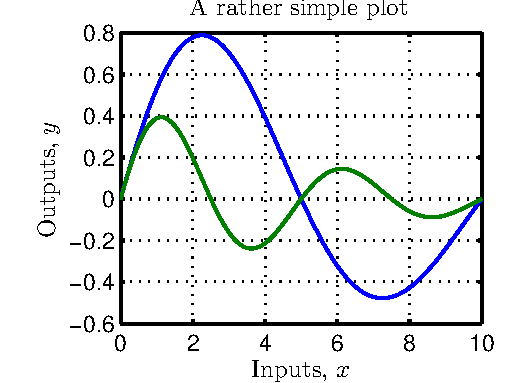
\includegraphics{simple_plot/figure_matlab.pdf}
\end{center}

\subsection{Matlab + export \_fig package + PDF backend}
\begin{center}
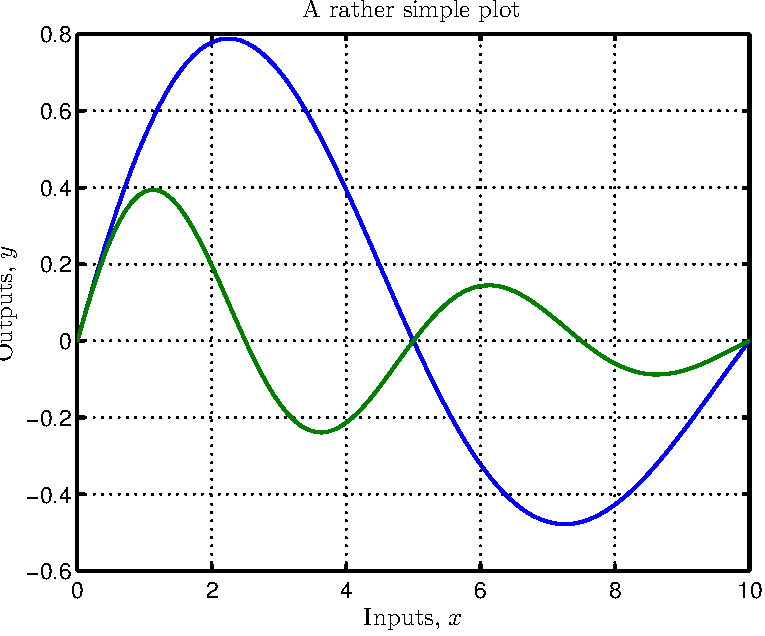
\includegraphics{simple_plot/figure_matlab_export_fig.pdf}
\end{center}

\subsection{Matlab + matlab2tikz package}
\begin{center}
% This file was created by matlab2tikz.
% Minimal pgfplots version: 1.3
%
%The latest updates can be retrieved from
%  http://www.mathworks.com/matlabcentral/fileexchange/22022-matlab2tikz
%where you can also make suggestions and rate matlab2tikz.
%
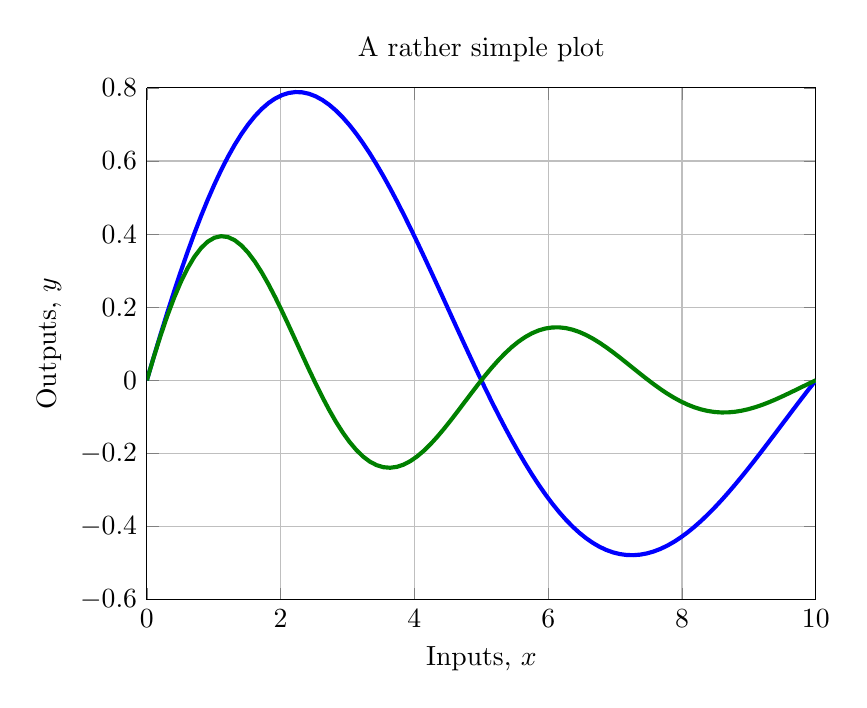
\begin{tikzpicture}

\begin{axis}[%
width=8.49518cm,
height=6.5cm,
at={(0cm,0cm)},
scale only axis,
separate axis lines,
every outer x axis line/.append style={black},
every x tick label/.append style={font=\color{black}},
xmin=0,
xmax=10,
xtick={ 0,  2,  4,  6,  8, 10},
xlabel={Inputs, $x$},
xmajorgrids,
every outer y axis line/.append style={black},
every y tick label/.append style={font=\color{black}},
ymin=-0.6,
ymax=0.8,
ytick={      -0.6,       -0.4,       -0.2, 1.1102e-16,        0.2,        0.4,        0.6,        0.8},
ylabel={Outputs, $y$},
ymajorgrids,
title={A rather simple plot}
]
\addplot [color=blue,solid,line width=1.5pt,forget plot]
  table[row sep=crcr]{%
0	0\\
0.101010101010101	0.0627864987208066\\
0.202020202020202	0.124060689746267\\
0.303030303030303	0.183602379292711\\
0.404040404040404	0.241202858356924\\
0.505050505050505	0.296665526060478\\
0.606060606060606	0.349806451039415\\
0.707070707070707	0.400454869823906\\
0.808080808080808	0.448453621431034\\
0.909090909090909	0.493659517670129\\
1.01010101010101	0.535943648932884\\
1.11111111111111	0.575191625508647\\
1.21212121212121	0.611303754728103\\
1.31313131313131	0.644195154494678\\
1.41414141414141	0.673795804011824\\
1.51515151515152	0.700050532754941\\
1.61616161616162	0.722918948968047\\
1.71717171717172	0.742375309186912\\
1.81818181818182	0.758408330501375\\
1.91919191919192	0.77102094746933\\
2.02020202020202	0.780230015782869\\
2.12121212121212	0.786065964962628\\
2.22222222222222	0.788572402519334\\
2.32323232323232	0.787805672170883\\
2.42424242424242	0.783834368839667\\
2.52525252525253	0.776738813276581\\
2.62626262626263	0.766610489266663\\
2.72727272727273	0.753551446464815\\
2.82828282828283	0.737673671989747\\
2.92929292929293	0.719098433969416\\
3.03030303030303	0.697955600281857\\
3.13131313131313	0.674382935772018\\
3.23232323232323	0.648525381247407\\
3.33333333333333	0.620534317563855\\
3.43434343434343	0.590566818107457\\
3.53535353535354	0.558784892959791\\
3.63636363636364	0.525354728002411\\
3.73737373737374	0.490445922171129\\
3.83838383838384	0.454230726015299\\
3.93939393939394	0.416883284647352\\
4.04040404040404	0.378578888089834\\
4.14141414141414	0.339493231935178\\
4.24242424242424	0.299801691134305\\
4.34343434343434	0.259678609619511\\
4.44444444444444	0.219296608348412\\
4.54545454545455	0.178825914228446\\
4.64646464646465	0.138433712247484\\
4.74747474747475	0.0982835229944399\\
4.84848484848485	0.0585346076059759\\
4.94949494949495	0.019341402022871\\
5.05050505050505	-0.0191470177173114\\
5.15151515151515	-0.056787437587232\\
5.25252525252525	-0.0934429736753208\\
5.35353535353535	-0.128983505057854\\
5.45454545454545	-0.163286070371763\\
5.55555555555556	-0.196235227194204\\
5.65656565656566	-0.227723373502972\\
5.75757575757576	-0.257651030663391\\
5.85858585858586	-0.285927087553406\\
5.95959595959596	-0.312469005606952\\
6.06060606060606	-0.33720298471895\\
6.16161616161616	-0.36006409011661\\
6.26262626262626	-0.380996340459151\\
6.36363636363636	-0.399952757581248\\
6.46464646464646	-0.416895378444016\\
6.56565656565657	-0.431795230000493\\
6.66666666666667	-0.444632267820049\\
6.76767676767677	-0.455395279447295\\
6.86868686868687	-0.464081753596032\\
6.96969696969697	-0.470697716395682\\
7.07070707070707	-0.475257536018891\\
7.17171717171717	-0.47778369712087\\
7.27272727272727	-0.47830654661634\\
7.37373737373737	-0.476864012406137\\
7.47474747474747	-0.473501296744286\\
7.57575757575758	-0.468270546005907\\
7.67676767676768	-0.461230498677594\\
7.77777777777778	-0.452446113444603\\
7.87878787878788	-0.441988179292954\\
7.97979797979798	-0.429932909579686\\
8.08080808080808	-0.416361522051021\\
8.18181818181818	-0.401359806806122\\
8.28282828282828	-0.385017684213044\\
8.38383838383838	-0.367428754785078\\
8.48484848484848	-0.348689843017847\\
8.58585858585859	-0.328900537171984\\
8.68686868686869	-0.308162726964478\\
8.78787878787879	-0.286580141098764\\
8.88888888888889	-0.264257886527864\\
8.98989898989899	-0.241301991299166\\
9.09090909090909	-0.217818952776489\\
9.19191919191919	-0.193915292980054\\
9.29292929292929	-0.169697122718245\\
9.39393939393939	-0.14526971611673\\
9.49494949494949	-0.120737097077342\\
9.5959595959596	-0.0962016391164428\\
9.6969696969697	-0.0717636799520695\\
9.7979797979798	-0.0475211521201942\\
9.8989898989899	-0.0235692308077818\\
10	1.44531498033966e-15\\
};
\addplot [color=black!50!green,solid,line width=1.5pt,forget plot]
  table[row sep=crcr]{%
0	0\\
0.101010101010101	0.0620303448731334\\
0.202020202020202	0.120601429178462\\
0.303030303030303	0.174903225519708\\
0.404040404040404	0.224226810715517\\
0.505050505050505	0.267971824466442\\
0.606060606060606	0.305651877364052\\
0.707070707070707	0.336897902005912\\
0.808080808080808	0.361459474484024\\
0.909090909090909	0.379204165250687\\
1.01010101010101	0.390115007891434\\
1.11111111111111	0.394286201259667\\
1.21212121212121	0.391917184419833\\
1.31313131313131	0.383305244633331\\
1.41414141414141	0.368836835994873\\
1.51515151515152	0.348977800140929\\
1.61616161616162	0.324262690623704\\
1.71717171717172	0.295283409053728\\
1.81818181818182	0.262677364001205\\
1.91919191919192	0.227115363007649\\
2.02020202020202	0.189289444044917\\
2.12121212121212	0.149900845567153\\
2.22222222222222	0.109648304174206\\
2.32323232323232	0.069216856123742\\
2.42424242424242	0.0292673038029879\\
2.52525252525253	-0.00957350885865572\\
2.62626262626263	-0.0467214868376604\\
2.72727272727273	-0.0816430351858816\\
2.82828282828283	-0.113861686751486\\
2.92929292929293	-0.142963543776703\\
3.03030303030303	-0.168601492359475\\
3.13131313131313	-0.190498170229575\\
3.23232323232323	-0.208447689222008\\
3.33333333333333	-0.222316133910025\\
3.43434343434343	-0.232040876798016\\
3.53535353535354	-0.237628768009446\\
3.63636363636364	-0.23915327330817\\
3.73737373737374	-0.236750648372143\\
3.83838383838384	-0.230615249338797\\
3.93939393939394	-0.220994089646477\\
4.04040404040404	-0.20818076102551\\
4.14141414141414	-0.192508842106522\\
4.24242424242424	-0.174344921508924\\
4.34343434343434	-0.154081363482239\\
4.44444444444444	-0.132128943263932\\
4.54545454545455	-0.108909476388245\\
4.64646464646465	-0.0848485613591223\\
4.74747474747475	-0.0603685485386712\\
4.84848484848485	-0.0358818399760347\\
4.94949494949495	-0.0117846154038909\\
5.05050505050505	0.0115489310312406\\
5.15151515151515	0.0337717703459742\\
5.25252525252525	0.0545685739709792\\
5.35353535353535	0.073659556862599\\
5.45454545454545	0.090803593744708\\
5.55555555555556	0.105800586879304\\
5.65656565656566	0.118493076720424\\
5.75757575757576	0.128767099390827\\
5.85858585858586	0.136552306941577\\
5.95959595959596	0.141821377643245\\
6.06060606060606	0.14458875395717\\
6.16161616161616	0.144908755214958\\
6.26262626262626	0.142873120282179\\
6.36363636363636	0.138608042509705\\
6.46464646464646	0.132270765017966\\
6.56565656565657	0.124045808773686\\
6.66666666666667	0.114140908986544\\
6.76767676767677	0.102782737078552\\
6.86868686868687	0.0902124858865711\\
6.96969696969697	0.0766813948948995\\
7.07070707070707	0.0624462902228938\\
7.17171717171717	0.0477652108955134\\
7.27272727272727	0.0328931886966724\\
7.37373737373737	0.0180782437577771\\
7.47474747474747	0.00355765208382255\\
7.57575757575758	-0.0104454654025625\\
7.67676767676768	-0.023725189880497\\
7.77777777777778	-0.0360954528591778\\
7.87878787878788	-0.0473922585888476\\
7.97979797979798	-0.0574754615830318\\
8.08080808080808	-0.0662300881290015\\
8.18181818181818	-0.0735671984769764\\
8.28282828282828	-0.079424293956532\\
8.38383838383838	-0.0837652804575967\\
8.48484848484848	-0.0865800064341554\\
8.58585858585859	-0.0878833997488278\\
8.68686868686869	-0.0877142331993711\\
8.78787878787879	-0.08613355339085\\
8.88888888888889	-0.0832228116870949\\
8.98989898989899	-0.0790817392586963\\
9.09090909090909	-0.0738260107182608\\
9.19191919191919	-0.0675847424903266\\
9.29292929292929	-0.0604978729079194\\
9.39393939393939	-0.0527134710791167\\
9.49494949494949	-0.0443850208563396\\
9.5959595959596	-0.0356687248080637\\
9.6969696969697	-0.0267208709920781\\
9.7979797979798	-0.0176953026189744\\
9.8989898989899	-0.00874102744289201\\
10	5.31701667284069e-16\\
};
\end{axis}
\end{tikzpicture}%
\end{center}

\newpage
\subsection{Tikz / Matlab2tikz + grid adjust}
\begin{center}
% PGF OPTIONS
\pgfplotsset{
             major grid style = {dashed, black},
             axis line style  = {black, line width = 1pt}                       
             }
% PLOT
\begin{tikzpicture}
  \begin{axis}
    [
    grid   = major,
    xlabel = {Inputs,  $x$},
    ylabel = {Outputs, $y$}, 
    title  = {A rather simple plot},
    width  = 90mm,
    height = 65mm,
    xmin = 0.,
    xmax = 10.,
    ymin = -.6,
    ymax = .8,
    %enlarge x limits = false,
    every x tick/.style = {color = black, thick},    
    ytick  = {-.6, -.4, -.2, 0., .2, .4, .6, .8},
    %enlarge y limits = false,
    every y tick/.style = {color = black, thick},        
    ]
    \addplot  [
              color      = blue,
              mark       = none,
              line width = 1pt
              ] 
             table [x index=0,y index=1,col sep=space] {simple_plot/data.csv};
    \addplot  [
              color      = teal,
              mark       = none,
              line width = 1pt
              ]
              table [x index=0,y index=2,col sep=space] {simple_plot/data.csv};
  \end{axis}
\end{tikzpicture}
\\
% This file was created by matlab2tikz.
% Minimal pgfplots version: 1.3
%
%The latest updates can be retrieved from
%  http://www.mathworks.com/matlabcentral/fileexchange/22022-matlab2tikz
%where you can also make suggestions and rate matlab2tikz.
%

\pgfplotsset{
             major grid style = {dashed, black},
             axis line style  = {black, line width = 1pt}                       
             }

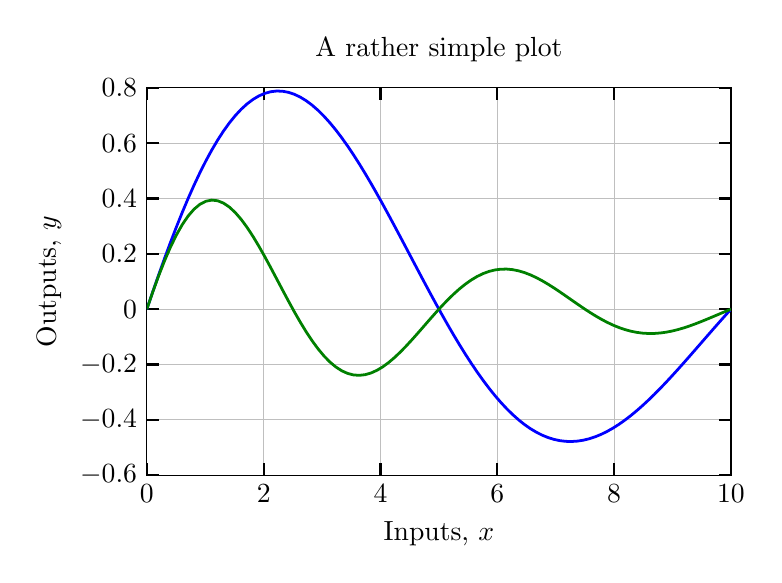
\begin{tikzpicture}

\begin{axis}[%
grid   = major,
width=9cm,
height=6.5cm,
at={(0cm,0cm)},
%scale only axis,
%separate axis lines,
every x tick/.style = {color = black, thick}, 
%every outer x axis line/.append style={black},
%every x tick label/.append style={font=\color{black}},
xmin=0,
xmax=10,
xtick={ 0,  2,  4,  6,  8, 10},
xlabel={Inputs, $x$},
%xmajorgrids,
%every outer y axis line/.append style={black},
%every y tick label/.append style={font=\color{black}},
every y tick/.style = {color = black, thick},        
ymin=-0.6,
ymax=0.8,
ytick={      -0.6,       -0.4,       -0.2, 0,        0.2,        0.4,        0.6,        0.8},
ylabel={Outputs, $y$},
%ymajorgrids,
title={A rather simple plot}
]
\addplot [color=blue,solid,line width=1pt,forget plot]
  table[row sep=crcr]{%
0	0\\
0.101010101010101	0.0627864987208066\\
0.202020202020202	0.124060689746267\\
0.303030303030303	0.183602379292711\\
0.404040404040404	0.241202858356924\\
0.505050505050505	0.296665526060478\\
0.606060606060606	0.349806451039415\\
0.707070707070707	0.400454869823906\\
0.808080808080808	0.448453621431034\\
0.909090909090909	0.493659517670129\\
1.01010101010101	0.535943648932884\\
1.11111111111111	0.575191625508647\\
1.21212121212121	0.611303754728103\\
1.31313131313131	0.644195154494678\\
1.41414141414141	0.673795804011824\\
1.51515151515152	0.700050532754941\\
1.61616161616162	0.722918948968047\\
1.71717171717172	0.742375309186912\\
1.81818181818182	0.758408330501375\\
1.91919191919192	0.77102094746933\\
2.02020202020202	0.780230015782869\\
2.12121212121212	0.786065964962628\\
2.22222222222222	0.788572402519334\\
2.32323232323232	0.787805672170883\\
2.42424242424242	0.783834368839667\\
2.52525252525253	0.776738813276581\\
2.62626262626263	0.766610489266663\\
2.72727272727273	0.753551446464815\\
2.82828282828283	0.737673671989747\\
2.92929292929293	0.719098433969416\\
3.03030303030303	0.697955600281857\\
3.13131313131313	0.674382935772018\\
3.23232323232323	0.648525381247407\\
3.33333333333333	0.620534317563855\\
3.43434343434343	0.590566818107457\\
3.53535353535354	0.558784892959791\\
3.63636363636364	0.525354728002411\\
3.73737373737374	0.490445922171129\\
3.83838383838384	0.454230726015299\\
3.93939393939394	0.416883284647352\\
4.04040404040404	0.378578888089834\\
4.14141414141414	0.339493231935178\\
4.24242424242424	0.299801691134305\\
4.34343434343434	0.259678609619511\\
4.44444444444444	0.219296608348412\\
4.54545454545455	0.178825914228446\\
4.64646464646465	0.138433712247484\\
4.74747474747475	0.0982835229944399\\
4.84848484848485	0.0585346076059759\\
4.94949494949495	0.019341402022871\\
5.05050505050505	-0.0191470177173114\\
5.15151515151515	-0.056787437587232\\
5.25252525252525	-0.0934429736753208\\
5.35353535353535	-0.128983505057854\\
5.45454545454545	-0.163286070371763\\
5.55555555555556	-0.196235227194204\\
5.65656565656566	-0.227723373502972\\
5.75757575757576	-0.257651030663391\\
5.85858585858586	-0.285927087553406\\
5.95959595959596	-0.312469005606952\\
6.06060606060606	-0.33720298471895\\
6.16161616161616	-0.36006409011661\\
6.26262626262626	-0.380996340459151\\
6.36363636363636	-0.399952757581248\\
6.46464646464646	-0.416895378444016\\
6.56565656565657	-0.431795230000493\\
6.66666666666667	-0.444632267820049\\
6.76767676767677	-0.455395279447295\\
6.86868686868687	-0.464081753596032\\
6.96969696969697	-0.470697716395682\\
7.07070707070707	-0.475257536018891\\
7.17171717171717	-0.47778369712087\\
7.27272727272727	-0.47830654661634\\
7.37373737373737	-0.476864012406137\\
7.47474747474747	-0.473501296744286\\
7.57575757575758	-0.468270546005907\\
7.67676767676768	-0.461230498677594\\
7.77777777777778	-0.452446113444603\\
7.87878787878788	-0.441988179292954\\
7.97979797979798	-0.429932909579686\\
8.08080808080808	-0.416361522051021\\
8.18181818181818	-0.401359806806122\\
8.28282828282828	-0.385017684213044\\
8.38383838383838	-0.367428754785078\\
8.48484848484848	-0.348689843017847\\
8.58585858585859	-0.328900537171984\\
8.68686868686869	-0.308162726964478\\
8.78787878787879	-0.286580141098764\\
8.88888888888889	-0.264257886527864\\
8.98989898989899	-0.241301991299166\\
9.09090909090909	-0.217818952776489\\
9.19191919191919	-0.193915292980054\\
9.29292929292929	-0.169697122718245\\
9.39393939393939	-0.14526971611673\\
9.49494949494949	-0.120737097077342\\
9.5959595959596	-0.0962016391164428\\
9.6969696969697	-0.0717636799520695\\
9.7979797979798	-0.0475211521201942\\
9.8989898989899	-0.0235692308077818\\
10	1.44531498033966e-15\\
};
\addplot [color=black!50!green,solid,line width=1pt,forget plot]
  table[row sep=crcr]{%
0	0\\
0.101010101010101	0.0620303448731334\\
0.202020202020202	0.120601429178462\\
0.303030303030303	0.174903225519708\\
0.404040404040404	0.224226810715517\\
0.505050505050505	0.267971824466442\\
0.606060606060606	0.305651877364052\\
0.707070707070707	0.336897902005912\\
0.808080808080808	0.361459474484024\\
0.909090909090909	0.379204165250687\\
1.01010101010101	0.390115007891434\\
1.11111111111111	0.394286201259667\\
1.21212121212121	0.391917184419833\\
1.31313131313131	0.383305244633331\\
1.41414141414141	0.368836835994873\\
1.51515151515152	0.348977800140929\\
1.61616161616162	0.324262690623704\\
1.71717171717172	0.295283409053728\\
1.81818181818182	0.262677364001205\\
1.91919191919192	0.227115363007649\\
2.02020202020202	0.189289444044917\\
2.12121212121212	0.149900845567153\\
2.22222222222222	0.109648304174206\\
2.32323232323232	0.069216856123742\\
2.42424242424242	0.0292673038029879\\
2.52525252525253	-0.00957350885865572\\
2.62626262626263	-0.0467214868376604\\
2.72727272727273	-0.0816430351858816\\
2.82828282828283	-0.113861686751486\\
2.92929292929293	-0.142963543776703\\
3.03030303030303	-0.168601492359475\\
3.13131313131313	-0.190498170229575\\
3.23232323232323	-0.208447689222008\\
3.33333333333333	-0.222316133910025\\
3.43434343434343	-0.232040876798016\\
3.53535353535354	-0.237628768009446\\
3.63636363636364	-0.23915327330817\\
3.73737373737374	-0.236750648372143\\
3.83838383838384	-0.230615249338797\\
3.93939393939394	-0.220994089646477\\
4.04040404040404	-0.20818076102551\\
4.14141414141414	-0.192508842106522\\
4.24242424242424	-0.174344921508924\\
4.34343434343434	-0.154081363482239\\
4.44444444444444	-0.132128943263932\\
4.54545454545455	-0.108909476388245\\
4.64646464646465	-0.0848485613591223\\
4.74747474747475	-0.0603685485386712\\
4.84848484848485	-0.0358818399760347\\
4.94949494949495	-0.0117846154038909\\
5.05050505050505	0.0115489310312406\\
5.15151515151515	0.0337717703459742\\
5.25252525252525	0.0545685739709792\\
5.35353535353535	0.073659556862599\\
5.45454545454545	0.090803593744708\\
5.55555555555556	0.105800586879304\\
5.65656565656566	0.118493076720424\\
5.75757575757576	0.128767099390827\\
5.85858585858586	0.136552306941577\\
5.95959595959596	0.141821377643245\\
6.06060606060606	0.14458875395717\\
6.16161616161616	0.144908755214958\\
6.26262626262626	0.142873120282179\\
6.36363636363636	0.138608042509705\\
6.46464646464646	0.132270765017966\\
6.56565656565657	0.124045808773686\\
6.66666666666667	0.114140908986544\\
6.76767676767677	0.102782737078552\\
6.86868686868687	0.0902124858865711\\
6.96969696969697	0.0766813948948995\\
7.07070707070707	0.0624462902228938\\
7.17171717171717	0.0477652108955134\\
7.27272727272727	0.0328931886966724\\
7.37373737373737	0.0180782437577771\\
7.47474747474747	0.00355765208382255\\
7.57575757575758	-0.0104454654025625\\
7.67676767676768	-0.023725189880497\\
7.77777777777778	-0.0360954528591778\\
7.87878787878788	-0.0473922585888476\\
7.97979797979798	-0.0574754615830318\\
8.08080808080808	-0.0662300881290015\\
8.18181818181818	-0.0735671984769764\\
8.28282828282828	-0.079424293956532\\
8.38383838383838	-0.0837652804575967\\
8.48484848484848	-0.0865800064341554\\
8.58585858585859	-0.0878833997488278\\
8.68686868686869	-0.0877142331993711\\
8.78787878787879	-0.08613355339085\\
8.88888888888889	-0.0832228116870949\\
8.98989898989899	-0.0790817392586963\\
9.09090909090909	-0.0738260107182608\\
9.19191919191919	-0.0675847424903266\\
9.29292929292929	-0.0604978729079194\\
9.39393939393939	-0.0527134710791167\\
9.49494949494949	-0.0443850208563396\\
9.5959595959596	-0.0356687248080637\\
9.6969696969697	-0.0267208709920781\\
9.7979797979798	-0.0176953026189744\\
9.8989898989899	-0.00874102744289201\\
10	5.31701667284069e-16\\
};
\end{axis}
\end{tikzpicture}%
\end{center}
\newpage

\end{document}